\documentclass[tikz]{standalone}
\usepackage{makecell}

\begin{document}

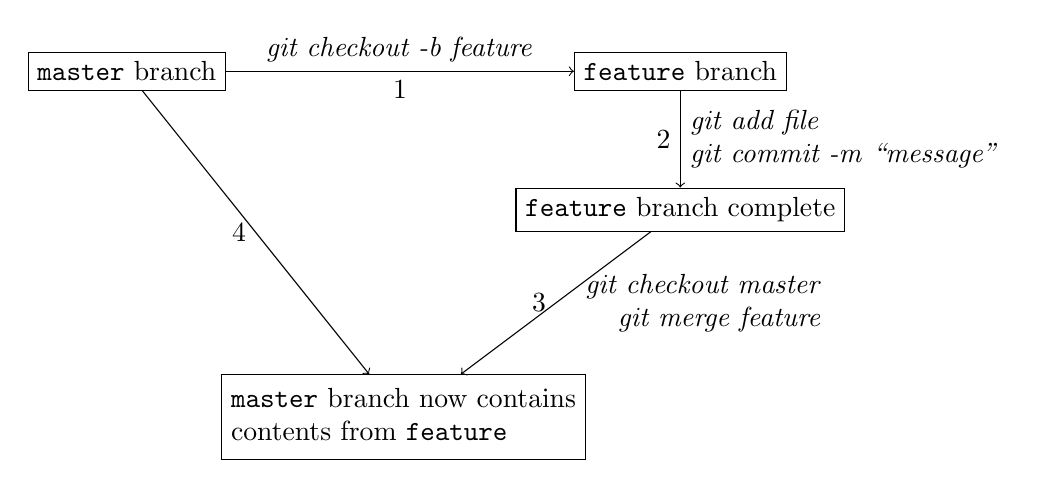
\begin{tikzpicture}
	\node[] at (-100pt, 0pt) [rectangle,draw] (master) {\texttt{master} branch};
	\node[] at (100pt, 0pt) [rectangle,draw] (feature) {\texttt{feature} branch};
	\draw[->] (master)  -- node[below]{1} node[above] {\emph{git checkout -b feature}} (feature);
	\node[] at (100 pt, -50pt) [rectangle,draw] (featuredone) {\texttt{feature} branch complete};
	\draw[->] (feature)  -- node[left]{2} node[right] {\makecell[l]{\emph{git add file}\\\emph{git commit -m ``message"}}} (featuredone);
	\node[] at (0pt, -125pt) [rectangle,draw] (merged) {\makecell[l]{\texttt{master} branch now contains\\contents from \texttt{feature}}};
	\draw[->] (featuredone) -- node[left]{3} node[right] {\makecell[r]{\emph{\ \ git checkout master}\\\emph{git merge feature}}} (merged);
	\draw[->] (master) -- node[left]{4} (merged);
\end{tikzpicture}

\end{document}
